%\documentclass{article} % Or some other class?  like 'report' or 'IEEEtran'
\documentclass[conference]{IEEEtran}
\usepackage[utf8]{inputenc}  
\usepackage{graphicx}        
\usepackage{cite} 
\usepackage{amsmath, amssymb}
\usepackage{hyperref}        
%\usepackage{natbib}       
\usepackage[colorinlistoftodos]{todonotes}
\usepackage{booktabs}
\usepackage{soul}        
\usepackage{svg}
\usepackage{hyperref}  
\usepackage{cleveref}

\newcommand\Mycite[1]{%             
  \citeauthor{#1}~\cite{#1}} 
% Produce citation in style     John et al. [1]         using \Mycite{}
% for citations in style        John et al. [2020]      change line 16 to    \citeauthor{#1}~[\citeyear{#1}]} 
  
\def\BibTeX{{\rm B\kern-.05em{\sc i\kern-.025em b}\kern-.08em
    T\kern-.1667em\lower.7ex\hbox{E}\kern-.125emX}}
    
\begin{document}

\title{To Block Or Not To Block? Evaluating Parental Controls Across Routers, DNS Services, and Software}


\author{\IEEEauthorblockN{Matteo Liberato}
\IEEEauthorblockA{University of Twente\\
m.liberato@utwente.nl}}

\author{\IEEEauthorblockN{Antonia Affinito}
\IEEEauthorblockA{University of Twente\\
a.affinito@utwente.nl}}

\author{\IEEEauthorblockN{Bernd Meijerink}
\IEEEauthorblockA{University of Twente\\
bernd.meijerink@utwente.nl}}

\author{\IEEEauthorblockN{Ralph Holz}
\IEEEauthorblockA{University of M\"{u}nster\\
ralph.holz@uni-muenster.del}}

\author{\IEEEauthorblockN{Mattijs Jonker}
\IEEEauthorblockA{University of Twente\\
m.jonker@utwente.nl}}

\author{\IEEEauthorblockN{Alessio Botta}
\IEEEauthorblockA{Universit\`{a} degli Studi di Napoli Federico II\\
a.botta@unina.it}}

\author{\IEEEauthorblockN{Anna Sperotto}
\IEEEauthorblockA{University of Twente\\
a.sperotto@utwente.nl}}


\author{\IEEEauthorblockN{Anonymous Authors}}


\maketitle

\begin{abstract}
In today's society, ensuring the safety of children online has become a priority for parents, educators, and policymakers. Parental control systems are widely used to restrict access to age-inappropriate online content, offering a tool for protecting children from potential online risks.
However, their blocking behavior across different technologies remains hidden and poorly analyzed.
In this paper, we present a comparative analysis of seven parental control solutions: three provided by routers with built-in filtering functionalities (TP-Link, Netgear, and ASUS), two DNS-based services (OpenDNS and DNS.eu), and a software tool (Norton Family).
Each system was tested by systematically visiting a large set of domains and recording which were blocked.
We then classified all domains into content categories and used this classification to evaluate the consistency and selectivity of each parental control system.
Our findings show that parental controls frequently fall short of providing adequate protection: Some systems fail to block up to 96\% of inappropriate domains, while others block appropriate content or apply inconsistent and arbitrary filtering rules.
For example, ASUS allows access to over 95\% of gambling websites, and Netgear exhibits internal inconsistencies, with one-third of the domains blocked under its "Adult" settings remaining accessible under its stricter "Child" setting.
These results provide insight into the real-world operation of popular parental control technologies and show a methodology for evaluating category-based filtering at scale.
\end{abstract}

\begin{IEEEkeywords}
Network measurements, Use and digitalization, Parental control.
\end{IEEEkeywords}

% Each parts automatically adds .tex to the input field

\section{Introduction}
% Go and look what I wrote on the SOK in the section about parental control?
% How specific should this section be? 

The Internet has become an integral part of children’s lives, offering a variety of educational resources, entertainment, and opportunities for social interaction.
However, this increased digital presence comes with significant risks.
%\todo[inline]{Anna: Changed the sentence ``Children are potentially exposed to harmful content, online predators, privacy invasions, and cyberbullying.'' into the one below, otherwise it would bring up the question of why listing those specific 4 threats and not other.}
Children are exposed to a wide range of online risks, including age-inappropriate content, online predators, privacy invasions, and cyberbullying. 
These dangers are documented in numerous studies and reports, such as those by UNICEF\cite{mariya_stoilova_investigating_2021} and Amnesty International\cite{amnesty_driven_2023}.
In response, a wide range of parental control tools have become available, promising to safeguard children by filtering inappropriate content, monitoring online activities, setting time restrictions and blocking access to age-inappropriate websites.
% These tools are widely used, according to a Pew Research Center report\cite{turner_parenting_2020}, over 70\% of parents of young children in the U.S. report using some form of parental control.
While parental control systems are an attractive solutions for parents, their effectiveness is difficult to verify due to a lack of transparency in how they operate. 
Many parental control solutions present themselves as tools capable of addressing a wide range of risks, but they often function as black-box systems, operating while hiding their internal functioning. 
As a consequence, users remain unaware of which content is being filtered, how filtering decisions are made, and whether these tools truly fulfill their promises. 
This lack of transparency raises concerns about the actual protection provided, including the risk of under-blocking (where harmful sites remain accessible) and potential over-blocking (where legitimate sites are restricted), affecting user's trust.
%\todo[inline]{Anna: the paragraph before is very well done!}

%\todo[inline]{NOT SURE WETHER TO KEEP THIS MENTION OF THE SOK; Anna @Matteo: I think we do not need it. You already motivated your work above, and there will be the RW section for what the literature says} 
%\st{In previous work, we conducted a systematization of knowledge (SOK) on online risks faced by children and the available mitigation strategies, including parental control technologies. 
%We focused on solutions grounded(?) in computer science, particularly those involving data science and network analysis. 
%Our findings highlighted a gap between what parental control tools claim to achieve and what is known about their real-world performance.
%This gap motivated the present study, where we focus on the network-level operations of parental control solutions, investigating the techniques used by different providers and their effectiveness.}

This paper aims to empirically analyze how parental control systems operate, focusing on their content blocking mechanisms and their blocking effectiveness.
Our study spans a range of deployment types, including consumer routers, DNS-based services, and software solutions, to represent the diversity of tools currently available to families.

% \todo[inline]{Anna: about the following sentences and the contributions: why is it important to differentiate between routers+DNS and software? It does make your story more complicated. Happy to talk about this}
%\hl{Our analysis revealed that many of these functionalities, including content blocking and filtering, rely heavily on the Domain Name System (DNS) protocols.}
%\hl{DNS filtering is a widely used technique in online security, where access to websites is controlled by intercepting and modifying DNS queries, often applied for blocking malicious websites or filtering inappropriate content (SOURCE). 
%By capturing and analyzing packet traces (PCAPs) of DNS traffic, we aim to understand how these services block content, their accuracy, and their potential limitations.
%DNS filtering, while effective, can lead to over-blocking, where legitimate content is unnecessarily restricted, or under-blocking, where harmful content slips through. 
%Furthermore, since DNS requests are often intercepted or redirected by parental control systems, understanding how these tools manipulate DNS traffic is essential for assessing their impact on user safety.
%On top of this we purchased subscirptions to two popular parental controls software solutions, Mobicip and Norton, to analyze their working(?) and measure their performance.
%Unlike routers and DNS providers, these software did not exhibit clear and regular markers of network-level blocking.
%Further analysis revealed that Norton relies on browser extensions to display block pages, while Mobicip installs its own root certificate and signs all visited websites, regardless of whether they are blocked or not.
%This behaviour indidcates that these tools may function as local or transparent proxies, though this remains speculative, judging on the traffic patterns and empirical behaviour that we observed.}
%\todo[inline]{Anna: the highlighted part is not needed for the introduction. There might be parts useful for other parts in the paper, so keep the text in comments}

\todo[inline]{Anna @all: we need to revise those contributions once the results are in to ensure consistency}
The contributions of this work are as follows:
\begin{itemize}
    \item We conduct an empirical analysis of parental control mechanisms implemented in three consumer routers, two DNS-based filtering services, and one software solution, using network traffic data collected during domain access attempts.
    \item We evaluate the behavior of each system on a pre-classified list of popular domains, identifying what content is blocked and inconsistencies or anomalies in the blocking logic.
    \item We document the techniques these systems appear to use for filtering, such as DNS manipulation, keyword matching, and application-level interception, and reflect on their transparency and reliability.
    % appear to due to the fact that we don't knwo about norton
\end{itemize}


This paper is organized as follows:
Section~\ref{sec:rw} provides background information and reviews relevant literature on parental control technologies. 
Section~\ref{sec:methodology} details our experimental setup and data collection process, while in 
Section~\ref{sec:dataset} we describe the domain list used to evaluate blocking behavior. 
In Section~\ref{sec:results}, we present our findings on how different systems implement filtering and what types of content they block. 
Section~\ref{sec:discussion} discusses the limitations of our study.
Finally, Section~\ref{sec:conclusions} presents our conclusions.  

\section{Background \& Related work}\label{sec:rw}
\subsection{Parental Controls}
Parental control tools are designed to assist parents in monitoring and managing their children’s online activities, with the goal of protecting children from potential online risks.
Risks include exposure to harmful content, cyberbullying, and excessive screen time, as such risks can impact children's cognitive, emotional, and social development \cite{livingstone_4cs_2021}.

Prior work has categorized online risks using the ``4Cs'' framework (Content risk, Contact risk, Conduct risk, and Contract risk).
This framework is used to distinguish between exposure to harmful material, interaction with potentially dangerous individuals, engagement in risky behavior, and privacy issues or commercial exploitation~\cite{livingstone_4cs_2021, bik_classifying_2023}.
Parental control tools can help mitigate these risks, targeting content categories such as pornographic or violent content, hate speech, and drug or gambling-related websites. 
These are frequently highlighted in risk taxonomies studies as high-priority threats to children online~\cite{alqahtani_state_2017, machado_fernandes_taxonomy_2022}.
%While parental control tools do not have a universal categorization system, these topics are widely considered key targets for most parental control tools.

Parental control tools typically include features such as content filtering, time management, and tracking the location and activities of specific devices. They can be deployed on various platforms (e.g. computers, mobile devices, video games consoles, and televisions), and in this case they are called \emph{device-specific} controls. If the controls target a specific application on a device (e.g. a browser), we talk about \emph{application-specific} controls. Finally, we have \emph{network-based} controls, which aim at blocking undesirable activity (e.g. requests to an unappropriated website) at the network level. This class of parental control is implemented, for example, on a router or by specialized software. This paper focuses on network-based parental controls and their content-filtering functionalities.
% They are available in different forms of implementations, including network-level solutions (such as ISP or router-based parental controls) and software applications installed directly on specific devices.

% Like other forms of Internet censorship \todo[inline]{Antonia: Can it be a little strong to say that? In any case, references about parental control deployment are needed. I do not get the rest.}, parental controls can be deployed in different parts of the network topology, both on the user side (e.g. parental control software installed on a device) or in the service side of the communication (e.g. ISP and DNS)\cite{rfc9505}.

%ANNA removed because it is a long repetition of what said before, then we go even in more details into Network-based
% Parental controls can be generally classified into three main types:
% \begin{itemize}
% 	\item Device-specific controls, which apply settings across an entire device (e.g., apps installed by parents in children's phones that monitor or restrict internet access)
% %
% 	\item Application-specific controls, which limit content within specific applications (e.g., Youtube restricting inappropriate videos on children's accounts).
% %
% 	\item Network-specific parental controls, provided by routers, DNS services or ISPs, that enforce content restrictions at the network level.
% \end{itemize}
% 


\subsection{Network-Based Parental Controls}
Network-based parental controls are a subset of parental controls that can be implemented using a variety of techniques. 
% They can be provided as a service by routers, ISPs or even external companies, such as Cloudflare, which offers a DNS service with built-in filtering features.
These solutions typically rely on methods such as IP blocking, URL filtering, Deep Packet Inspection (DPI) and DNS filtering\cite{noauthor_overview_nodate}. 
Each method serves a different purpose in restricting access to online content. IP-based blocking blocks traffic to specific IP addresses.
However, this method can be overly broad, as many unrelated websites may share the same IP, leading to possibly significant overblocking.
URL-based filtering inspects the full web address (URL) being accessed and blocks or allows the request based on a filter list.
It is more precise than IP blocking but requires deeper traffic inspection, which can be hindered by encryption.
Deep Packet Inspection (DPI) inspects not only the headers but also the content of packets to identify content to be blocked. While precise, DPI is resource-intensive and privacy-invasive. A different approach, DNS filtering, act on the Domain Name System, a fundamental service that translates human-readable domain names into numerical IP addresses, enabling users to access websites. 
DNS filtering works by intercepting DNS queries and modifying the responses (DNS injection), blocking access to restricted websites by preventing the resolution of their DNS queries.
This technique is relatively easy to implement and can be done at various levels, including public, ISP, and open DNS resolvers, making it a versatile tool for content control\cite{cheng_-depth_2022}.





\subsection{Related work}

Despite the increasing availability of parental control tools, the adoption rate remains relatively low \cite{ardito_designing_2021}.
For instance, the internation survey Global Kids Online shows that parental controls are used by less than 3\% of parents in several countries, and EU Kids Online data showed usage ranging from 11\% to around 33\% across European nations\cite{stoilova_parental_2024}.
% Over 50\% of children own a smartphone by age 11, yet only a fraction of parents use parental control solutions, most commonly in the form of device-based applications (Usability, security and privacy)~\cite{sun_are_2023}.
The reasons for this low adoption rate are multiple, including the balance between security, privacy and usability.
Parental control tools are at times perceived as difficult to use, too invasive or ineffective \cite{ardito_designing_2021}.
In addition, these tools often operate as black-box systems, offering limited insight into their operations, including which types of content are blocked and how such content is identified\cite{ali_betrayed_2020}.
The lack of transparency raises concerns about the actual protection provided and the overall impact on user trust. While recent tools increasingly integrate AI, edge computing, and cloud-based monitoring to improve filtering accuracy and usability\cite{razak_piwall_2024, ramezanian_parental_2021}, these advancements do not fully resolve the conflict between functionality, transparency, and privacy.
In this paper, we investigate the blocking behavior of parental controls, in particular focusing on over-blocking or under-blocking of content.
% In fact, many parental control solutions continue to exhibit security and privacy vulnerabilities, including opaque data practices, potential information leakage, and susceptibility to adversarial misuse\cite{ali_betrayed_2020}.

% The broader field of parental control has received more attention in terms of user experience and effects on family dynamics, often in the form of user-focused surveys. 
% For example, Stoilova et al.~\cite{stoilova_parental_2024} shows that real-world adoption remains low, often due to usability challenges.
% Similarly, Iftikhar et al.~\cite{ardito_designing_2021} highlights how design complexity and privacy concerns influence adoption decisions.
% Wang et al.~\cite{wang_protection_2021} examines how the design of mobile parental control apps influences user perceptions, focusing on feedback mechanisms, transparency, and parent-child communication.
% These studies show the importance of usability and design in shaping the effectiveness of parental control tools.

The broader field of parental control has received attention in terms of user experience and effects on family dynamics, often in the form of user-focused surveys \cite{stoilova_parental_2024,ardito_designing_2021,wang_protection_2021}
However, to the best of our knowledge, only a limited number of studies have examined how parental controls work from a technical point of view. 
Ali et al.~\cite{ali_parental_2021} investigates the security and privacy risks of various parental control implementations, including router-based solutions.
Feal et al.~\cite{feal_angel_2020} reveals serious privacy and security flaws in mobile parental control tools and Ali et al.~\cite{ali_betrayed_2020} claims to be the first comprehensive study analyzing different parental control solutions across multiple platforms.
These findings highlight how parental control internal mechanisms remain poorly explored and evaluated.
This work aims to addresses this gap by a network-level analysis of their real-world behavior.



At the technical level, several of the approaches supporting network-based parental control have been investigated in the context of other application areas.
%\todo[inline]{Ale: There are a couple of cases in which you refer to citations as subjects or objects, which I think is not very correct. For examples, the sentence: "Works like~\cite{feal-tnsm-2021, ramanathan-imc-2020, li-pam-2021, metcalf-wiscs-2015} investigated ..." should be something like: "The use and characteristics of IP-based blocklists has been investigated~\cite{feal-tnsm-2021, ramanathan-imc-2020, li-pam-2021, metcalf-wiscs-2015}"}
Works like~\cite{feal-tnsm-2021, ramanathan-imc-2020, li-pam-2021, metcalf-wiscs-2015} investigated the use and characteristics of IP-based blocklists. Feal et al.~\cite{feal-tnsm-2021} investigate 2093 free and open source IP-based blocklists to gain a better understanding about, among others, their coverage, liveliness and scope. Ramanathan et al.~\cite{ramanathan-imc-2020} focus on the interplay between IP-blocking and IP address reuse, arguing that IP-based blocking could lead to un-intended blocking of legitimate users. The work of Li at al.~\cite{li-pam-2021} uses network measurements to infer the use of IP blocklists in the wild. URL filtering and DPI are often studied in the context of Internet censorship, as for example in ~\cite{rfc9505,bock-usenix-2021, dalek-imc-2013, mcdonald-imc-2018}. Bock et al.~\cite{bock-usenix-2021} report that censorship middleboxes can react to TLS server name indication (SNI) fields. At the DNS level, a recent study by Liu et al~\cite{liu-ndss-2024} investigate the security implications of relying on protective DNS services, namely DNS resolvers that implement content filtering. Our paper also includes DNS-based filtering, but focuses instead on the filtering of content harmful to young Internet users. DNS-filtering has also been studied in the context of newer DNS implementations (e.g. DoH~\cite{vekshin_doh_2020}) and to assess the risk of content underblocking~\cite{cheng_-depth_2022}, or overblocking~\cite{hoang_how_2021,hoang_measuring_2022}.
%URL filtering
%DPI
%DNS FILTERING



% This approach is effective as it is lightweight and does not require installation on the user's device. 
% However, DNS-based research found that DNS filtering have limitations:

% - Over-blocking and under-blocking: Studies have shown that DNS filtering can fail to block access to certain content (underblocking)\cite{cheng_-depth_2022}, while DNS injection can also cause collateral damage, interfering with unrelated queries\cite{ververis_understanding_2015}.

% - Avoidance techniques: Encrypted DNS protocols such as DNS over HTTPS (DoH) and DNS over TLS (DoT) can allow users to bypass DNS-based filtering mechanisms by encrypting the content of DNS requests\cite{vekshin_doh_2020, bock-usenix-2021}.

% - Alternative resolvers:  Certain open DNS resolvers may remain unaffected even when local DNS filtering is enforced, reducing the reliability of this kind of control\cite{cheng_-depth_2022}.
% %(INTERNET SOCIETY PERSPECTIVES ON INTERNET CONTENT BLOCKING) CAN BE GOOD FOR MORE MATERIAL ON BLOCKING IN GENERAL

% While DNS filtering is common in router-based parental controls and DNS is widely researched in many of its aspects, including its use for censorship\cite{cheng_-depth_2022}, there is a lack of published research comparing how different parental control providers implement filtering policies.
% There is a substantial body of work analyzing DNS-based filtering as a mechanism for online content control, particularly in the context of national-level censorship.
% Studies such as Hoang et al.~\cite{hoang_how_2021}, Cheng et al.~\cite{cheng_-depth_2022} and Hoang et al.~\cite{hoang_measuring_2022} show that DNS filtering systems are prone to overblocking, inconsistent enforcement, and circumvention. 
% However, these studies largely focus on censorship regimes or national infrastructure. 
% There is comparatively little peer-reviewed work examining how DNS filtering is implemented specifically within  parental control tools.
  

\section{Methodology}\label{sec:methodology}
Parental controls are typically marketed with generic claims about their functionalities, promising to protect children while providing no information about their functioning.
To investigate their actual implementations and effectiveness, we examined the consumer market for parental control solutions across hardware, software and the DNS. 
% We compiled a list of parental controls solutions from routers with integrated parental control features and software products to test on Windows devices.
% \todo[inline]{They could ask why we did not include \st{DNS}, ISPs and browsers in this point. Anna: indeed. We need to add a sentence in RW about considering ISP and browsers out of scope}
To try and ensure broad coverage and relevance we aimed to identify devices and services that are likely to be adopted by actual families. 
Our selection was guided by three criteria:

\begin{enumerate}
\item Popularity, which we determined trough user reviews and ratings (considering both the amount of reviews and the score) on retail platforms such as Amazon. 
\item  Market relevance, recognized from mentions in consumer-focused rankings (e.g. blog-posts about the best parental controls of the year on technology forums) and professional reviews.
\item Diversification, aiming to include major providers to reflect the available commercial offerings, rather than focusing on a single vendors solutions.
\end{enumerate}

%\begin{table*}[!t]
 %   \centering
  %  \begin{tabular}{|c|c|}
   % \hline
    % \textbf{Solution} & \textbf{Type} \\
     %\hline
     %TP-Link (Archer AX10) & Router \\
     %\hline
     %Netgear (Nighthawk series ADD EXACT MODEL) & Router \\
     %\hline
     %ASUS (RT-AX56U) & Router \\
     %\hline
     %Norton Family & Software \\
     %\hline
     %OpenDNS FamilyShield & DNS \\
     %\hline
     %DNS.eu & DNS \\
     %\hline
    %\end{tabular}
    %\caption{Parental control solutions considered in the study}
    %\label{tab:parental_controls}
%\end{table*}


From this process, we selected three router solutions, one software solution and two DNS-based filtering mechanisms, which are summarized in Table~\ref{tab:parental_controls}.

\begin{table}[htbp]
	\centering
    \begin{tabular}{|c|c|}
    \hline
    \textbf{Solution} & \textbf{Type} \\
    \hline
    TP-Link (Archer AC1900) & Router \\
    \hline
    Netgear (Nighthawk AX5400) & Router \\
    \hline
    ASUS (RT-AX57) & Router \\
    \hline
    Norton Family & Software \\
    \hline
    OpenDNS FamilyShield & DNS \\
    \hline
    DNS.eu & DNS \\
    \hline
    \end{tabular}
    \vspace{0.5\baselineskip} 
    \caption{Parental control solutions analyzed in the study}
    \label{tab:parental_controls}
\end{table}
    
    

% From this process, we selected three routers from three different manufacturers: TP-Link (Archer AX10), Netgear (Nighthawk series ADD EXACT MODEL), and ASUS (RT-AX56U).
% On the software side trough the same process we selected Norton Family.
%\todo[inline]{Anna: Check the commented paragraph in here, some of the text can be used in the RW.}
% While our initial focus was on hardware-based parental controls, early tests on the ASUS router revealed that its filtering mechanism relied on external DNS services.
% Based on this observation, we decide to extend our analysis to include examples of DNS-based parental control services, which apply filtering at the resolver level.
% As a result, we added OpenDNS FamilyShield and DNS.eu Kids to our evaluation.
% These resolvers are commonly used in private, professional or institutional networks to restrict access to inappropriate or dangerous websites.
% Their inclusion allowed us to compare router-level filtering with dedicated DNS services, using the same Tranco domain list.

%\todo[inline]{Anna: we need to check if we want to keep this here or if we want to have a separate subsection.}
To evaluate how each parental control system handles different types of content, we 
designed our tests around a popularity list of domains (see Sec.~\ref{sec:dataset}) and the set of identified parental control solutions. To identify which domains should be blocked by a parental control, we rely on content categories, such as porn and gambling, using domain classification data (see Sec.~\ref{sec:dataset}).
In particular, we tested how each solution blocks or allows each of the domains in the popularity list. Since we expected the selected solutions to have different blocking methodologies (e.g. DNS or HTTPS), we used different approaches targeting the specific solutions. We therefore first define a behaviour baseline for each solution (See ~\ref{sec:results-baseline}).

%  list derived from the Tranco dataset\footnote{\url{https://tranco-list.eu/}}.
% Tranco aggregates the most visited websites across multiple popularity rankings (including Cisco Umbrella, and Majestic), and provides the top 1M popular domains list updated daily.
% This dataset forms the basis of our tests, enabling us to analyze filtering behavior across a wide range of websites.
% Within the Tranco dataset, we identified content inappropriate for minors (e.g., pornography, gambling) using the classification provided by Cisco Umbrella. 
% (add link and short explanation of what Cisco did)
% A more detailed discussion of this classification process appears in Sec.~\ref{sec:dataset}.

Each of the identified solutions necessitates of a specific data collection methodology, which we explain in the following subsections.


\subsection{Routers}
To analyze how each router implements its parental control functionalities, we built a controlled environment involving three physical routers and three dedicated client PCs. Each PC is connected via LAN to one router.
Each router is connected to the Internet via its WAN port, allowing it to resolve DNS queries and apply filtering policies as it would in a real-world scenario.
To capture and analyze traffic, we tapped both the LAN and WAN connections:
The LAN capture records the traffic sent by the client PC to the router and the router's responses.
The WAN capture monitors traffic between the router and the Internet, including DNS lookups and connections to web servers.

\begin{figure}[htbp]
    \centering
    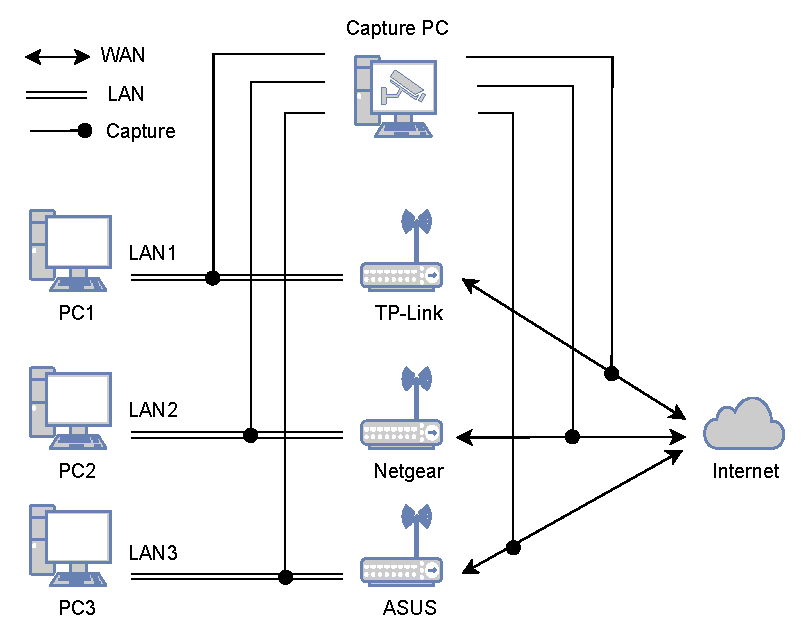
\includegraphics[width=0.9\linewidth]{Images/Methodology/capture.pdf}
    \caption{Capture setup to investigate the behaviour of the routers.}
    \label{fig:capture}
\end{figure}

This setup, shown in Figure~\ref{fig:capture}, gives us an overview of the traffic entering and exiting each router. 
We captured PCAPs of each connection and used Wireshark to analyze them and extract information about the behaviour of the routers.
By comparing what is sent by the PC and what is allowed to leave (or blocked) by the router, we can observe exactly how each device enforces its parental control policies, especially at the DNS level.
%On the computer, these tunnels are linked to different virtual networks (VLANs), each one assigned to a specific port on a switch.
%Each of those switch ports is connected to the WAN port of a different router (TP-Link, Netgear, ASUS).
%With this setup the VM can send traffic directly to each router as if it were a regular Internet connection.
%At the same time, each router’s LAN port is connected back to the switch on another set of ports. 
%These ports use different VLANs, and the desktop sends that traffic back through tunnels to the same VM. 
%This way, the VM sees both the traffic toward the router (trough the WAN) and what comes out of it (trough the LAN), letting us monitor how the router modifies each request.
% This setup lets us automate the testing of the routers parental control functionalities while keeping the communications under control.
Each router was tested with parental controls enabled and disabled, allowing us to isolate and understand the specific blocking behavior.
% We initially ran the tests with full HTTP/HTTPS browsing, but we realized that the resulting PCAPs were too large for scalable analysis.
% We then developed a lightweight testing script that performs only DNS lookups (via a --noHttp flag), greatly reducing traffic volume while still capturing blocking behavior.

\subsubsection{The TP-Link case}
The TP-Link router uses a set of user-defined keywords as base for its filtering mechanisms. This implies that we need to initialize such a set before conducting our experiments. In this case, we tried to put ourselves in the shoes of a parent confronted with such a task, and we therefore asked ChatGPT to create a list of keywords (31 words, as this is the maximum allowed by TP-Link), based on a set of website categories of inappropriate or harmful content (see Sec.~\ref{sec:dataset}).

\subsection{Software}
For software-level parental controls, we analyzed Norton Family. 
We installed the software solution on a Windows machine. We iterate over the input list of domains using a curl script and we monitored the outgoing traffic using Wireshark to collect possible evidence of blocking behaviour.  

%ANTONIA move to results
% Our initial approach was similar to the one used for the routers, capturing PCAPs using Wireshark during browsing sessions. 
% However, Norton was not suited for this type of measurement. 
% We observed inconsistent signs of activity, such as failed TLS handshakes, or unexplained delays. 
% These artifacts were not regular or reliable enough to support a large scale measurement.
% For this reason, we developed an alternative detection strategy.
% After exploring several approaches, including monitoring the behavior of the browser extensions installed by Norton, we settled on a curl-based script.
% This script visits each domain and determines whether it is blocked by analyzing the resulting HTML content.
%Specifically, the script looks for known indicators of a Norton block page, such as the presence of the word “NortonLifeLock” and references to the logo file used in the block page.

% Mobicip functions as a \st{certification authority} transparent proxy, installing its own root certificate and intercepting all HTTPS traffic at the local device level.
% To reliably detect which domains were being blocked, we developed an automated testing script using Playwright (https://playwright.dev/), an open-source tool for controlling browsers.
% We used it to run a headless browser, meaning a browser that operates without a visible user interface, 
% This approach is good for large-scale automated testing since it consumes fewer resources and has faster execution time, compared to a full browser session.
 
\subsection{DNS}
% {WE ALREADY EXPLAINED WHY WE ADDED THESE SERVICES, SHOULD I ADD MORE AS AN INTRODUCTION. Anna: no I think this is enough at the moment
% descritto separatamente va bene (e.g. nella subsection DNS), ma nell'introduzione e nella parte introduttiva della metodologia direi semplicemente quello che abbiamo scelto, non come ci siamo arrivati}
OpenDNS FamilyShield and DNS.eu Kids are publicly accessible DNS resolvers that advertise family-safe filtering.
To analyze their behavior, we created a measurement script that uses the dig to send DNS queries to each service.
%The script records the DNS response and classifies a domain as blocked if the response is empty (for DNS.eu Kids) or it contains a known block IP (\texttt{146.112.61.106} for OpenDNS).
We limited the number of daily queries sent to each service to prevent rate-limiting or automatic blocking.


  

\section{Dataset}\label{sec:dataset}
% \todo[inline]{MJ: In light of the methodology vs. data sources separation we agreed during the 26/03 meeting, I assume
% the following will have been discussed in the preceding methodology section:
% 1) We use a list of top ranked domain names to investigate how PCS behave
% across a diverse range of domains \ldots ({\bf without} already specifying
% Tranco); and 2) we identify content categories such as porn and gambling in the
% input domains using domain classification data ({\bf without} already
% specifying Cisco Umbrella Investigate API).}

In the following sections we provide details on our list of input domains and the classification data.

\subsection{List of Input Domains}
\label{sec:dataset:input_domains}

We use the Tranco Top 1 Million (downloaded on 19-02-2025, root domains) for our list of diverse input domains.
Tranco\footnote{\url{https://tranco-list.eu/}} is a research-oriented ranking
of the most-visited websites and includes domains spanning a variety of content
categories such as social media, news and search engines.
The list aggregates multiple other top lists, including Cloudflare Radar, the
Cisco Umbrella Popularity List, the Majestic Million, and the Crome User
Experience Report (CrUX). As Tranco aggregates these lists it addresses some of
their shortcomings, which include instability, inter-list disagreement, and
susceptibility to rank manipulation.
We use the standard version of the list with apex domains.
%\todo[inline]{MJ: to add: date(s)/snapshot(s) of Tranco list used. Readers may want to know.}

\subsection{Input Data for Domain Classification}
\label{sec:dataset:classification_data}

% \todo[inline]{MJ: from AA I understand that the Cisco API offers subdomain
% categorization. This raises a question: does PCS behavior change with subdomain granularity? If the
% answer is maybe, then, considering that you worked with Tranco root domains (while a subdomains list is also available), we need to
% probably describe as limitation that the findings are scoped to root-level domain behavior.}
% \todo[inline]{Anna: I added root domains to the Tranco paragraph, and add a few lines about this in the limitations}
%\todo[inline]{MJ: Let's avoid the term ``reclassification'' but rather use ``collate``, ``group`` and ``consolidate``}

We use the Cisco Umbrella Investigate API for domain name classification.
The \emph{domain status and categorization} data\footnote{\url{https://umbrella.cisco.com/products/umbrella-investigate}}
offers a detailed set of categories. To make these data more manageable and
relevant for evaluating parental controls, we developed a heuristic to
consolidate the categories into a smaller and simplified set. This
is guided by three key principles:

\begin{enumerate}
    \item We analyze the co-occurrence of categories across all input domains
        to identify cases where multiple categories are frequently assigned to
        the same domain (an example will follow in~\cref{sec:dataset:tranco_categories}).
        Such categories are candidates to be collated into a simpler category;
    \item We then collate similar and overlapping categories that provide additional
        granularity but no meaningful distinction in terms of web content
        filtering. For example, we merge \emph{Radio}, \emph{Music}, and
        \emph{Entertainment} into the simpler \emph{Entertainment};
    \item We consider categories through the specific lens of parental
        control system evaluation, and infer if a category should
        typically be blocked for children. For example, we expect the simpler \emph{Adult Content} category, which 
        collates Cisco categories such as \emph{Pornography} and \emph{Dating}, to not be meant for children.
\end{enumerate}

This results in a simplified, content-oriented classification that facilitates
the measurement of blocking behavior across different parental control
solutions.  The consolidated categories serve as the basis for our
exploration of which types of content are blocked by each parental control system.

\begin{figure}[!tb]
    \centering
    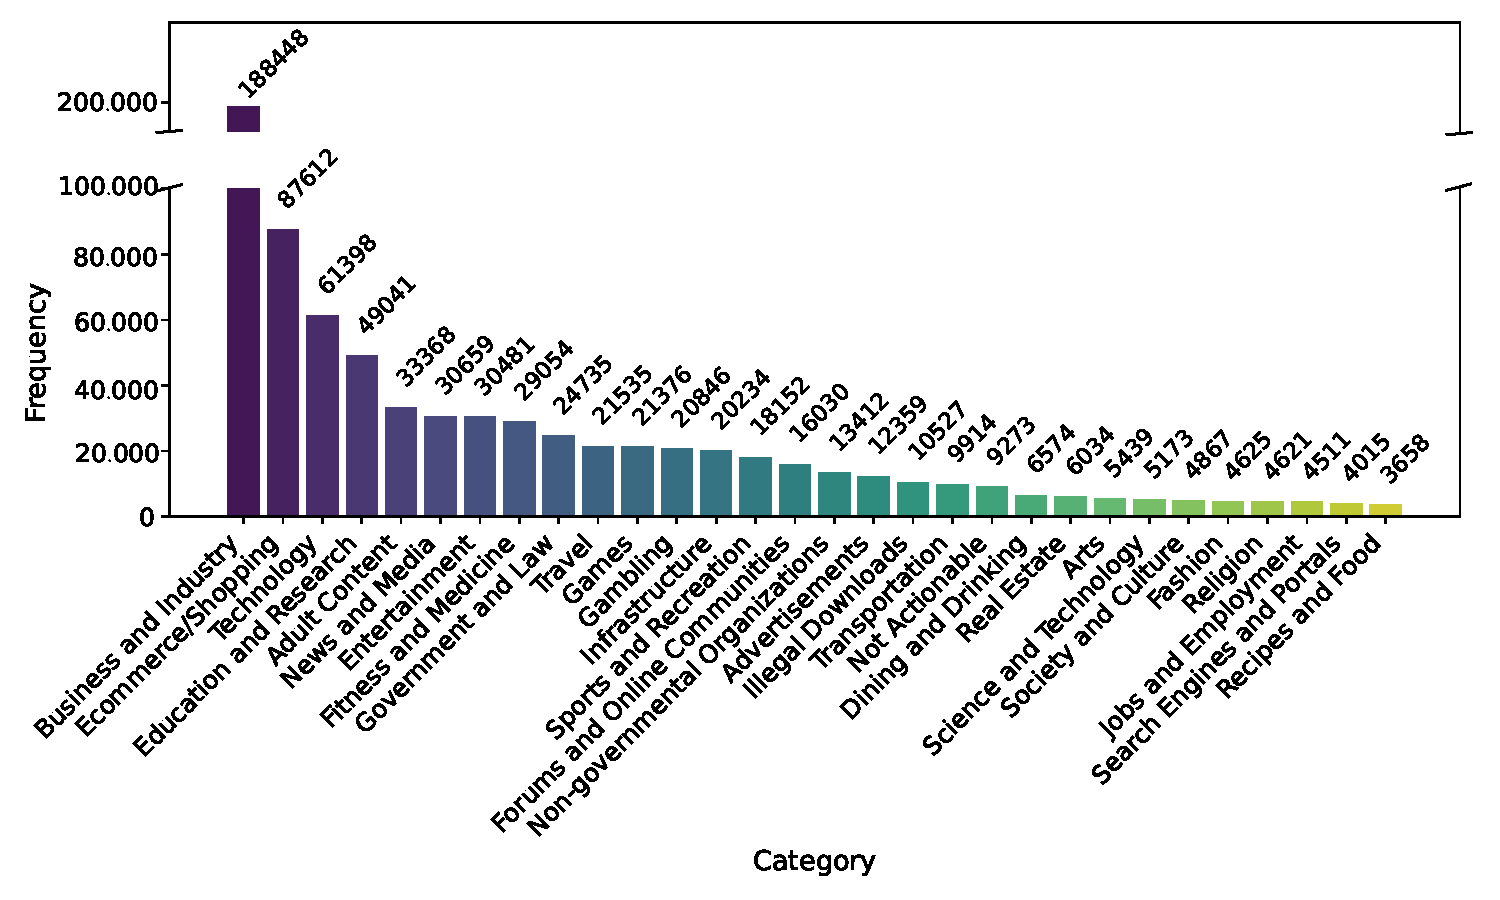
\includegraphics[width=1\columnwidth]{Images/top_30_categories.pdf}
    \caption{Tranco Lisy Top 30 Content Categories by Frequency.}
    \label{fig:top30categories}
\end{figure}

\subsection{Content Distribution Across Input Domains}
\label{sec:dataset:tranco_categories}

We mapped the Tranco list to categories to understand the distribution of content.
We were able to map 779,591 domains using the Cisco data. For the other 220,409 domains the Cisco data
does not offer a category.
%\todo{AA(?): we need to decide how to show these domains}
Figure\ref{fig:top30categories} shows the most prevalent categories among the Tranco domains.

Further analysis revealed that uncategorized domains appear more frequently
toward the long tail of the list. Only 8K domains missing a category are among
the Top 100K of the Tranco list.  We can only speculate as to the reasons for
this difference, but the position of domains in the list suggests that
categorization services may be more effective for high-traffic domains.
%, and may struggle with newly registered or obscure domains.

% \todo[inline]{AA: I think we need to make some analysis before making this claim; MJ: instead of analysis, is this something Cisco (or related work in this space) could confirm/support?}
% \todo[inline]{ML: This is not something that is based on anything i found in the literature, its pure speculation on my side simply based on the increasing number of unknown domains in the latter part of the list, if CISCO can confirm it ok, otherwise if the claim is too strong (even in this form) we will have to change it}
% \todo[inline]{Ale: The question is how excluding the non-ranked domains would impact the results? If we have restricted the blocking analysis to domains that have a cathegory, we can simply remove such a speculation and say something like "we concentrate on domains with a cathegory and we verified that domains without any cathegory are tipycally low ranking ones".}
% \todo[inline]{Anna: Answering Alessio: no, we did not restrict the analysis to having a category. I decided to tame down the claim by removing the part about struggling. The part about being more effective is speculative, but we are clear about it}

We next analyzed the extent to which domains were assigned multiple categories.
The vast majority of domains (95\%) mapped to a single class, with fewer than
4\% assigned two classes, and less than 0.5\% assigned three or more.
We conducted an analysis of category co-occurrences, which revealed that
several classes appeared together so frequently that they effectively
functioned as a single category, validating our intuition to collate and simplify categories.
For example, the \emph{Shopping} category co-occurred with
\emph{Ecommerce/Shopping} in 86,7K cases, while the prior appeared without the
latter fewer than 2K times.

By collating Cisco categories into simpler ones, we reduced the number of domains still assigned
multiple categories by several orders of magnitude, from hundreds
of thousands to a few thousand at most.
Of the consolidated categories, we consider \emph{Adult Content},
\emph{Gambling}, \emph{Hate/Discrimination} and \emph{Terrorism} to likely be
candidates for blocking by parental control systems. In the remaining of this paper, we will use those categories as reference for comparing the blocking capabilities of different solutions.
%\todo[inline]{AA: but we query all the domains, ?!}
In Figure~\ref{fig:blockedcategories} we show the cumulative distribution of
domains under these four categories in order of rank.
As shown, the number of domains belonging
to \emph{Hate/Discrimination} and \emph{Terrorism} is extremely low, while
\emph{Adult Content} and \emph{Gambling} are much more prevalent. In general, we observer that domains in these categories are quite evenly spread throughout the entire Tranco list.

\begin{figure}[!t]
    \centering
    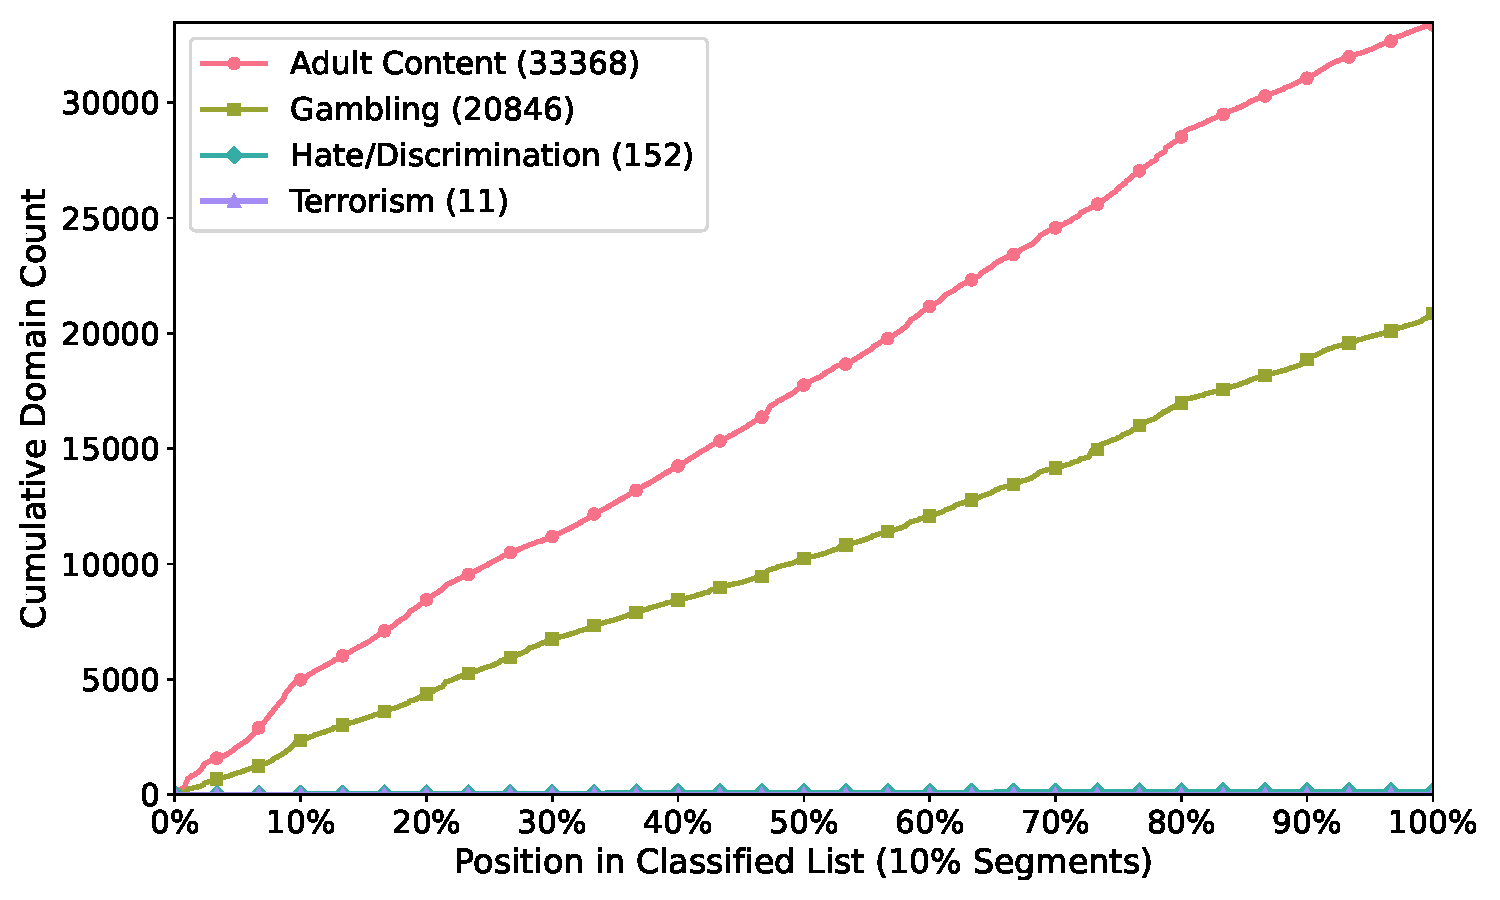
\includegraphics[width=0.95\columnwidth]{Images/cumulative_blocked_categories.pdf}
    \caption{Distribuion of Domains in Sensitive Categories.}
    \label{fig:blockedcategories}
\end{figure}

%\todo[inline]{AA: Increase the font size of the text in the figures.}
%\todo[inline]{AA(?): Update the numbers}
% \todo[inline]{Ale: I do not get the reason for this figure: why only these cathegorie? Do they sum up to the total number of domains considered? Using log scale for y axis would improve the visibility of the hate and terrorism. In general, a more detailed explanation is needed if we leave it.}
% \todo[inline]{Anna: I now explicitly added that we will use those categories as reference to measure the blocking capabilities. At least it makes sense to show something more about them in this way. I also added that they are evenly spread in the dataset. I know it is not very detailed}


\section{Results}\label{sec:results}
% h = here (try to place the figure exactly where the code appears)
% t = top (place it at the top of a page)
% b = bottom (place it at the bottom of a page)
% p = page of floats (place it on a separate page with just figures/tables)
% ! = override restrictions (e.g., \begin{figure}[!ht] tells LaTeX to try harder to place it here)
In this section, we present the results of our analyses. First, we show the baseline domain filtering analysis of all the parental control systems, providing insights into how each system blocks domains. Next, we show their overall blocking behavior and examine their blocking mechanisms by category, showing how each system handles different types of content.
 
\subsection{Baseline Domain Filtering} \label{sec:results-baseline}
%\todo[inline]{Ale: Do we report somewhere that we did not consdier dns over https?}
As outlined in Section \ref{sec:methodology}, we analyzed the PCAPs of each router’s LAN and WAN connections to assess their parental control mechanisms. We established a baseline for blocking behavior by testing HTTPS connections both with and without parental control. Our findings show that the routers do not apply HTTPS-based filtering. Instead, they rely on DNS-based filters, each using a different approach.

TP-Link, for instance, implements a basic keyword-based filter mechanism, blocking DNS queries that contain user-defined keywords. Our packet capture analysis confirms this behavior: such DNS queries are visible on the LAN connection between the computer and the router, but are absent on the WAN connection between the router and the Internet. This suggests that the router intercepts and drops these DNS requests before they are forwarded to the external network.
In contrast, Netgear uses a more advanced approach.
It intercepts DNS queries and validates them against an internal API at \emph{\url{https://urldb.meetcircle-netgear.co}}.
If a domain is flagged as inappropriate or harmful, the router blocks access by responding with an IP address from the \emph{10.123.0.0/16} range.
Additionally, this router allows users to fine-tune blocking with four protection levels: Child, Teen, Adult, and None.
ASUS, on the other hand, redirects all DNS queries to Cloudflare for Families (\emph{IP address: 1.1.1.3}) when parental control is enabled. 
If a domain is deemed inappropriate, Cloudflare for Families returns the IP address \emph{0.0.0.0} instead of the correct address, blocking access by preventing the resolution of the domain.
Based on our analysis, the decision on whether a domain is allowed or not is made entirely by the Cloudflare service.

Regarding the Norton software, our initial approach was similar to the one used for the routers, capturing PCAPs using Wireshark during browsing sessions. However, Norton was not suited for this type of measurement. We observed inconsistent signs of activity, such as failed TLS handshakes, or unexplained delays. These artifacts were not regular or reliable enough to support a large scale measurement. For this reason, we developed an alternative detection strategy. After exploring several approaches, including monitoring the behavior of the browser extensions installed by Norton, we settled on a curl-based script that determine if a domain is blocked by analyzing its HTML content. Specifically, we look for known indicators of a Norton block page, such as the presence of the term “NortonLifeLock” and references to the logo file used in the block page.

Finally, for the DNS resolvers, OpenDNS FamilyShield and DNS.eu Kids, we send a DNS query and record the response for domains from the Tranco list. A domain is classified as blocked if the response is empty (for DNS.eu Kids) or if it contains a known block IP address (\emph{146.112.61.106} for OpenDNS).


%\todo[inline]{Ale: The takeways are not clear to mme: they seem to mix the mechanisms used by routers/resovers/software to block access to inappropriate websites with the mechanisms we used to study them.}
\textit{Key takeaway: Routers and DNS resolvers implement parental control systems through DNS-based filters, involving user-defined keywords, external services, or redirecting to a blocking page. In contrast, software-based systems require analyzing the HTML content of the webpage. This attests the diversity of blocking methodologies among parental controls.}
%=======
%\textit{Key takeaway: Routers and DNS resolvers implement parental control systems through DNS-based filters, involving user-defined keywords, external services, or redirecting to a blocking page. In contrast, software-based systems require analyzing the HTML content of the webpage. This attests the diversity of blocking methodologies among parental controls.}
%>>>>>>> 4795dab (results and discussion)

\subsection{Overall Blocking Behavior}  \label{sec:results-overallblocking}

After analyzing the blocking mechanisms of each system, we evaluated the total number of domains blocked to assess their effectiveness in filtering inappropriate content. As shown in Figure~\ref{fig:blocked_domains}, Norton blocks 322,870 domains, significantly more than any other system, followed by DNS.eu with 132,045 blocked domains. %%%Check if it works like this
\begin{figure}
    \centering
    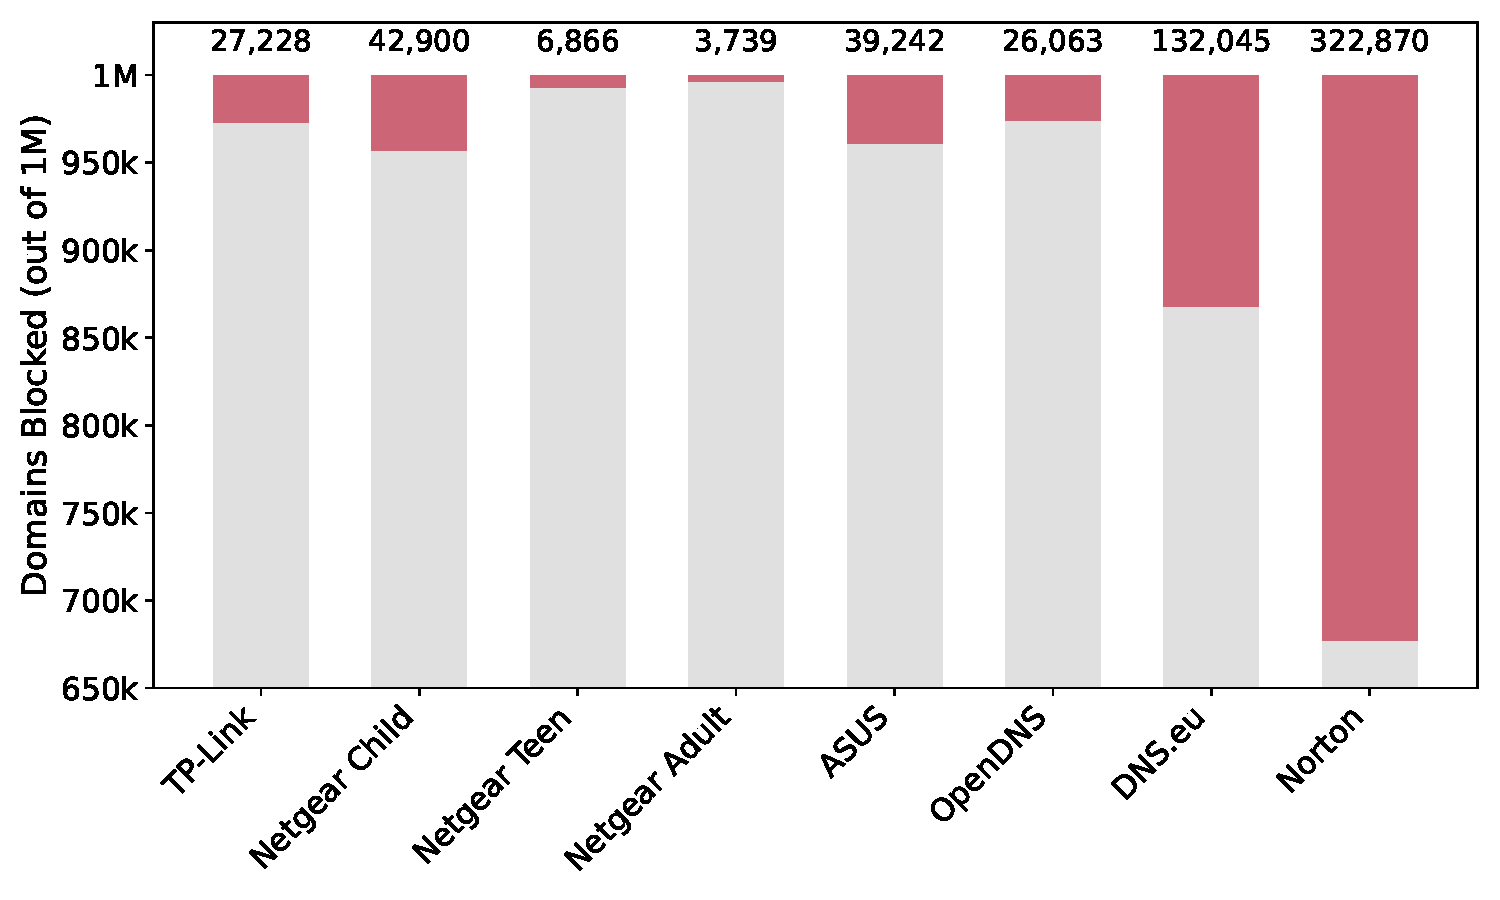
\includegraphics[width=0.85\columnwidth]{Images/Results/blocked_domains_per_tool.pdf}
    \caption{Total number of domains blocked by each parental control system.}
    \label{fig:blocked_domains}
\end{figure}
Netgear’s blocking behavior varies significantly depending on the setting. For example, in the Adult setting, it blocks fewer than 4k domains, while in the Child setting, it blocks over 10 times as many (42,900). The teen setting, on the other hand, blocks 6,866 domains.
The variation is expected, as these configurations are designed for different use cases. However, we also expected less variation between the Child and Teen settings than between the Teen and Adult settings, as both Child and Teen options are supposed to filter content for younger users, while the Adult option is typically less restrictive.
In comparison, ASUS blocks a closer number of domains (39,242) to the Netgear's child setting. TP-Link, which allows users to specify keywords to block, blocks approximately 27,228 domains, more than OpenDNS that blocks approximately 26,000 domains. As a result, OpenDNS blocks the fewest domains among the systems evaluated, excluding Netgear’s Teen and Adult filters.

\begin{table*}[htbp]
    \centering
    \resizebox{\textwidth}{!}{
    \begin{tabular}{lcccccccc}
    \toprule
    \textbf{Category (Total)} & \textbf{TP-Link} & \textbf{Netgear Child} & \textbf{Netgear Teen} & \textbf{Netgear Adult} & \textbf{ASUS} & \textbf{OpenDNS} & \textbf{DNS.eu} & \textbf{Norton} \\
    \midrule
    Business and Industry (188448) & 0.3\% & 1.7\% & 0.1\% & 0.1\% & 0.3\% & 0.1\% & 7.6\% & 17.8\% \\
    Ecommerce/Shopping (87612) & 0.4\% & 4.7\% & 0.1\% & 0.1\% & 0.5\% & 0.1\% & 2.3\% & 17.2\% \\
    Technology (61398) & 0.3\% & 2.5\% & 0.2\% & 0.2\% & 0.6\% & 0.2\% & 8.2\% & 23.5\% \\
    Education and Research (49041) & 0.2\% & 2.8\% & 0.1\% & 0.1\% & 0.4\% & 0.0\% & 6.8\% & 12.7\% \\
    \textbf{Adult Content (33368)} & \textbf{27.7\%} & \textbf{5.0\%} & \textbf{5.6\%} & \textbf{6.3\%} & \textbf{63.8\%} & \textbf{73.5\%} & \textbf{70.5\%} & \textbf{74.5\%} \\
    News and Media (30659) & 0.5\% & 28.2\% & 0.2\% & 0.1\% & 0.2\% & 0.1\% & 2.3\% & 12.7\% \\
    Entertainment (30481) & 0.5\% & 6.1\% & 0.4\% & 0.2\% & 5.0\% & 0.6\% & 4.9\% & 24.8\% \\
    Fitness and Medicine (29054) & 0.4\% & 13.4\% & 0.1\% & 0.0\% & 0.6\% & 0.0\% & 4.4\% & 15.6\% \\
    Government and Law (24735) & 0.2\% & 28.5\% & 0.1\% & 0.1\% & 0.1\% & 0.0\% & 11.2\% & 6.2\% \\
    Travel (21535) & 0.7\% & 1.2\% & 0.2\% & 0.0\% & 0.1\% & 0.1\% & 3.8\% & 9.4\% \\
    \midrule
    \multicolumn{9}{c}{\textellipsis} \\
    \midrule
    \textbf{Gambling (20846)} & \textbf{16.9\%} & \textbf{3.7\%} & \textbf{4.4\%} & \textbf{0.4\%} & \textbf{0.9\%} & \textbf{0.2\%} & \textbf{13.9\%} & \textbf{75.3\%} \\
    \textbf{Hate/Discrimination (152)} & \textbf{0.7}\% & \textbf{19.1\%} & \textbf{9.2\%} & \textbf{0.7}\% & \textbf{10.5\%} & \textbf{7.2\%} & \textbf{13.8\%} & \textbf{46.1\%} \\
    \textbf{Terrorism (11)} & \textbf{0.0}\% & \textbf{18.2\%} & \textbf{27.3\%} & \textbf{0.0}\% & \textbf{54.5\%} & \textbf{0.0}\% & \textbf{18.2\%} & \textbf{36.4\%} \\
    \bottomrule
    \end{tabular}}
    \vspace{0.5\baselineskip} 
    \caption{Percentage of domains blocked by each parental control system, for the most frequent categories in the Tranco list and the four sensitive categories.}
    \label{tab:blocked_categories}
\end{table*}

To further understand the nature of this blocking, we also examined the ranking of the blocked domains in the Tranco list, specifically assessing whether the systems prioritize blocking higher-ranked and potentially more popular domains.
This is important because blocking popular domains may have a greater impact on real-life user experience and exposure to content compared to blocking low-traffic sites.

Figure~\ref{fig:cdf_blocked_domains} shows the cumulative distribution function of blocked domains across the Tranco Top 1 million list. The logarithmic scale is used to highlight differences in blocking behavior across domains with different popularity levels.
The x-axis represents the domain rank, from most to the least popular, while the y-axis shows the cumulative number of blocked domains up to each rank, with the axis ending at the total of one million domains.



Netgear Child shows the highest concentration of blocked domains in the early ranks, with 50\% of its blocked domains appearing within the top 31\% of the Tranco list (rank 310,472), and 90\% reaching rank 826,542. This suggests that, despite its limited overall coverage, Netgear Child prioritizes blocking more popular domains. Similarly, Netgear Adult follows a comparable trend, with 50\% of its blocked domains reaching rank 329,750.
In contrast, Netgear Teen shows a more gradual distribution, with 50\% of its blocked domains appearing only by rank 472,049. This suggest that its filtering is more spread out across the ranking, giving less emphasis on popular domains compared to the other Netgar configurations.
In contrast, TP-Link shows a relatively flat progression, reaching 50\% of its blocked domains only by rank 629,440, and 90\% by rank 952,000. This pattern is not due to an inherent filtering policy but reflects the limitations of the keyword-based blocking mechanism. Since domains are blocked only if their names contain a blocklist term, this approach disproportionately affects lower-ranked or obscure domains, where such terms are more likely to appear.
Norton, despite its much larger blocking volume, shows a more gradual rise: half of its blocked domains appear by rank 650,143, and 90\% by 930,832. 
DNS.eu, OpenDNS  and ASUS reach the 50\% thresholds at ranks 430,748, 459,953 and 480,093 respectively, around middle of the Tranco list, indicating a more balanced focus between popular and unpopular domains.
On average, across all eight systems, 50\% of blocked domains appear by rank 470,331, and 90\% by 886,945, indicating that most tools concentrate their blocking in the lower half of the Tranco list.

%\textcolor{red}{Norton stands out with a steep and early curve, indicating that it blocks a large number of domains across the entire ranking spectrum, including many highly ranked sites. DNS.eu and OpenDNS follow a similar pattern, though with a smaller total volume, still focusing their blocking on both popular and mid-ranked domains.
%TP-Link, using keyword filtering, shows a relatively flat CDF with only occasional steps, confirming that its blocking is sparse and not biased toward high-ranking domains. 
%This is expected, keyword-based blocking tends to affect niche or less popular domains, rather than well-known, high-traffic sites with specific, proprietary domain names.
%Netgear, across all three configurations, shows very limited blocking throughout the ranking. 
%The curves for the Adult, Teen, and Child settings remain nearly flat, indicating that not only do they block few domains overall, but also fail to prioritize domains with higher visibility or traffic. 
%This further reinforces the earlier observation that Netgear's parental control features do not effectively target the most prominent or potentially impactful domains.
%Overall, the CDF reinforces the pattern observed so far: 
%DNS-based systems and Norton offer broad, visible filtering, while router-based tools are either too narrow in scope or fail to block inappropriate content even when it appears in popuar domains.}

\textit{Key takeaway: Among the different solutions, we observe a large variability in the number of blocked domains with variations in the range of 300k to 7k, which raise questions about the effectiveness of these solutions.}

\subsection{Domain Blocking Across Categories} \label{sec:results-categories}
%Netgear is the only system that provides distinct filtering levels: Child, Teen, and Adul. To explore how the blocking is applied across these levels, we trace how individual domains are classified across these settings to assess the logical consistency of its filtering features.



\begin{figure}[t]
    \centering
    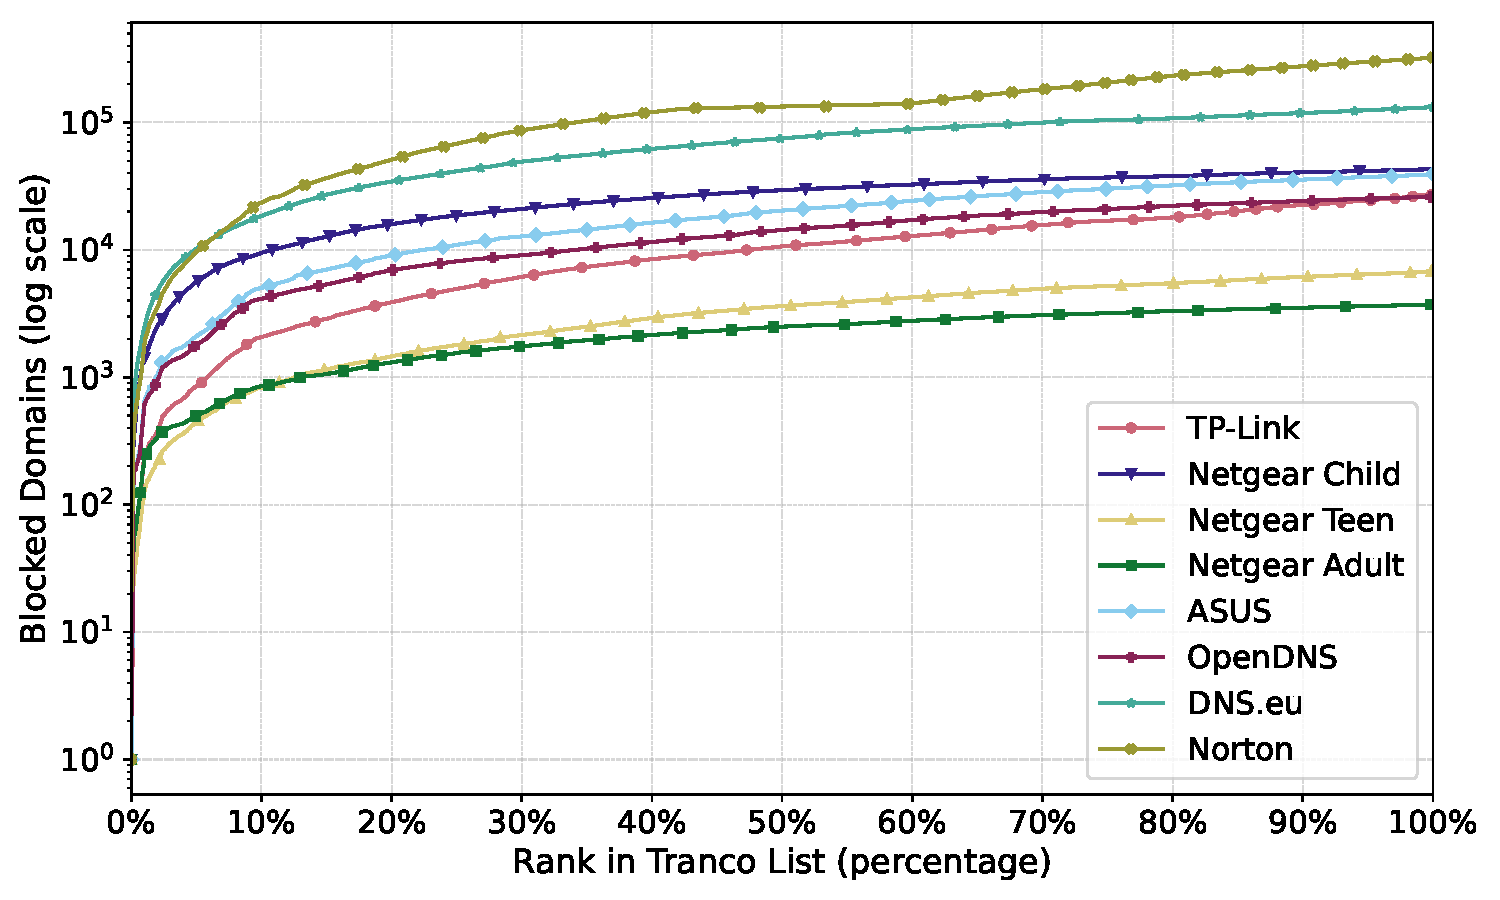
\includegraphics[width=0.85\columnwidth]{Images/Results/cdf_blocked_domains_log.pdf}
    \caption{Cumulative Distribution of Sensitive Domains Across the Tranco Top 1 million.}
    \label{fig:cdf_blocked_domains}
\end{figure}

To better understand the types of content most frequently blocked by each system, we evaluated the proportion of blocked domains across various content categories. We calculated the ratio of blocked domains in each category to the total number of domains in that category, as shown in Table~\ref{tab:blocked_categories}. Several notable patterns emerge, revealing strong differences in filtering priorities. We observe that systems like OpenDNS, DNS.eu, and Norton block a high percentage of domains across the sensitive category \emph{Adult Content}, with blocking rates of 73.5\%, 70.5\% and 74.5\% respectively. Additionally, Norton stands out as the system that blocks over 73\% of domains in the \emph{Gambling} category and achieves the highest blocking rates in \emph{Hate/Discrimination} and \emph{Terrorism}, further confirming its overall stricter filtering policy. 
However, on the other hand, Norton applies its broad filtering even to non-sensitive domains, blocking over 15\% of \emph{Education}, \emph{Technology}, and \emph{Business and Industry} sites, raising concerns about overblocking.

In contrast, router-based systems tend to block fewer domains and show more variability in their filtering across categories.
Notably, despite being the most restrictive among Netgear's settings, the Child configuration performs poorly in inappropriate categories, blocking only 5.0\% of \emph{Adult Content} and 3.7\% of \emph{Gambling} domains. Additionally, \emph{Hate/Discrimination} and \emph{Terrorism} categories are blocked at rates of 19.1\% and 18.2\%, respectively, which is relatively low. It is important to note that the \emph{Terrorism} category is very small (only 11 domains), so even slight differences in absolute blocking result in large percentage differences.
Instead, it blocks a larger percentage of non-sensitive domains, such as 28.2\% of \emph{News and Media}, 28.5\% of \emph{Government and Law}, and 13.4\% of \emph{Fitness and Medicine}, notable percentages for categories that typically would not require such strict filtering. This suggests a broad filtering strategy that fails to prioritize the inappropriate content typically expected from a parental control system.

%`` <quoted text here> '' 

ASUS, while more effective in targeting \emph{Adult Content} (63.8\%), shows limited blocking in other sensitive categories, suggesting a narrower and more focused approach.
Finally, TP-Link, as explained in Sec. \ref{sec:methodology}, blocks domains containing any of 31 user-defined keywords and performs well in categories such as \emph{Adult Content} (27.7\%) and \emph{Gambling} (16.9\%). This suggests that domains related to Adult Content and Gambling are more likely to contain keywords associated with those categories, such as ``bet''  or ``casino'', whereas domains in the Hate/Discrimination and Terrorism categories have entirely different names that do not include these keywords.

Overall, it appears that only DNS-based systems and Norton provide robust protection for categories commonly associated with harmful or inappropriate content, while router-based systems, particularly Netgear, struggle to effectively block these inappropriate domains.

\iffalse
\begin{figure}[htbp]
    \centering
    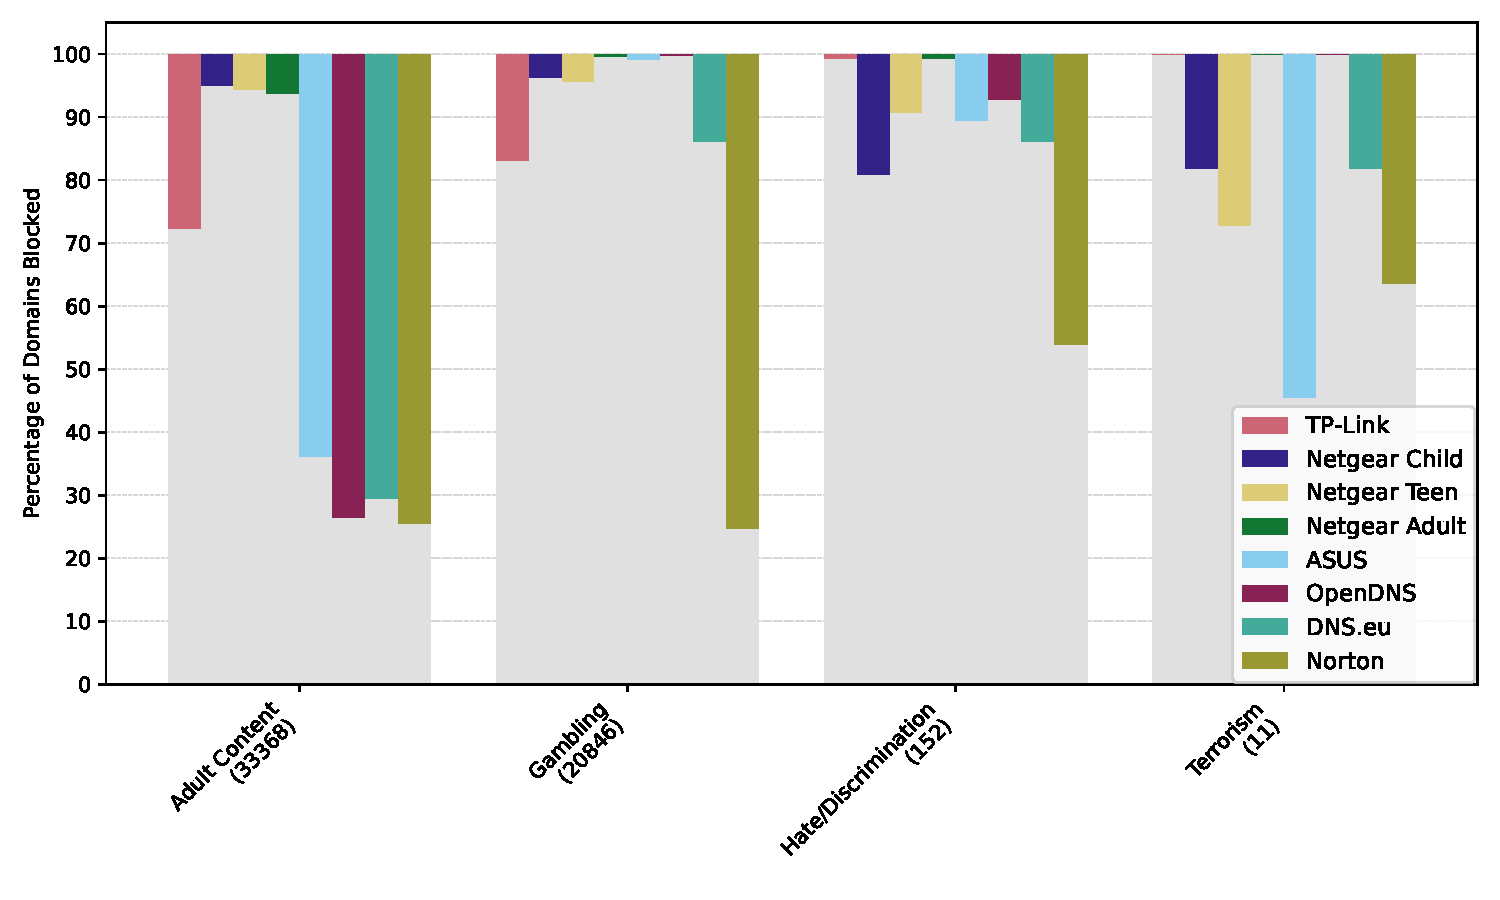
\includegraphics[width=0.85\columnwidth]{Images/Results/blocked_by_category.pdf}
    \caption{Percentage of domains blocked in four core sensitive categories: Adult Content, Gambling, Hate/Discrimination, and Terrorism.}
    \label{fig:blocked_by_category}
\end{figure}
\fi
%\textcolor{red}{Norton, DNS.eu, and OpenDNS consistently demonstrate the highest blocking rates, exceeding 70\% in Adult Content and Gambling, and maintaining strong blocking levels in Hate/Discrimination and Terrorism.
%ASUS shows strong filtering of Adult Content (63.8\%) but drops off sharply in the other categories, suggesting a narrow focus in the blocking policy.
%Netgear, even when using the Child setting, performs poorly across the board, blocking less than 6.5\% in any of the four categories.
%This is particularly problematic for Hate/Discrimination and Terrorism, which receive almost no attention. 
%Notably, while the Child setting is the most restrictive in terms of total domains blocked, it is not the most effective at blocking Adult Content or Gambling. 
%In fact, the Teen setting blocks slightly more Adult Content (5.6\%) than the Child setting (5.0\%), and the Adult setting blocks more Gambling (6.3\%) than both. 
%This pattern, opposite of what would be expected logically, suggests that the Child setting may apply broader but less targeted restrictions, failing to prioritize the most sensitive types of content.
%In contrast, the Teen and Adult settings appear to focus more narrowly on specific high-risk categories.
%However, the overall blocking rates remain low across all three settings, indicating that none of the Netgear configurations offer strong protection for these high-risk categories.
%As mentioned before TP-Link, guided solely by keyword matching, performs surprisingly well in Adult Content (27.7\%) and moderately in Gambling (16.9\%), but completely fails to capture Hate/Discrimination and Terrorism, where associated terms are unlikely to appear in domain names.
%It is important to note that the Terrorism category is very small (only 11 domains), so even slight differences in absolute blocking result in large percentage differences.
%Results regarding that category should be interpreted with caution.}




\begin{figure}[htbp]
    \centering
    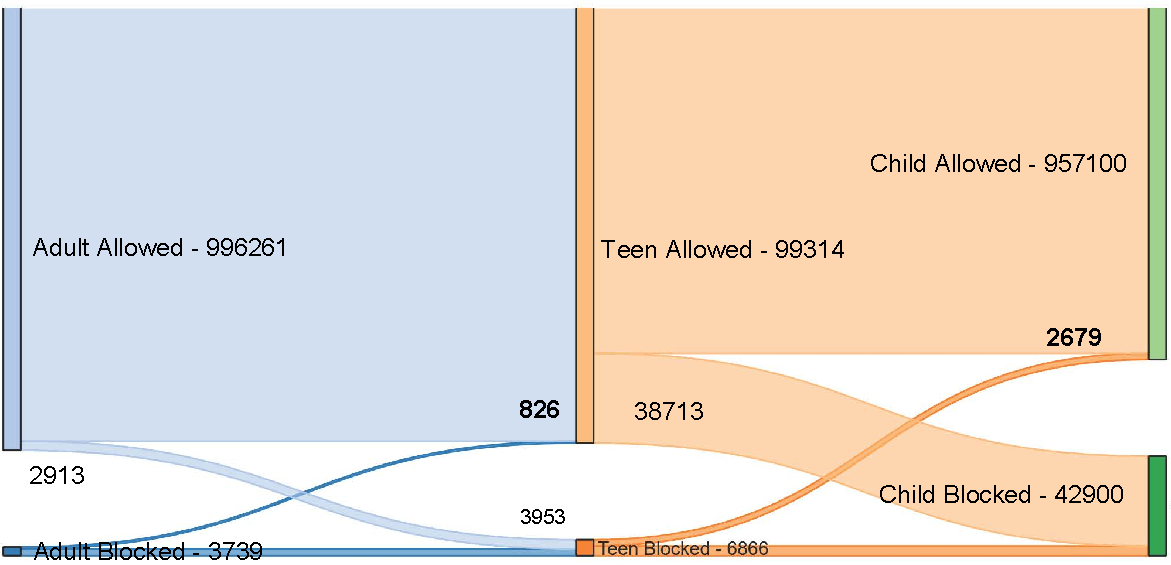
\includegraphics[width=0.95\columnwidth]{Images/Results/bokeh_plot.pdf}
    \caption{Domain Blocking Decisions Across Netgear's Child, Teen, and Adult configurations.}
    \label{fig:netgear_sankey}
\end{figure}

Figure~\ref{fig:netgear_sankey} shows the flow of domain blocking across the three Netgear’s parental control settings. 
Each column represents one of these settings, while the edges illustrate how domains are handled across different parental control levels.
At the Adult level, 3,739 domains are blocked, and 996,261 are allowed. Of the 3,739 domains blocked at the Adult level, most (2,913) remain blocked in the Teen setting, but 826 domains are unexpectedly allowed in Teen despite being blocked in Adult, which contradicts the expected progression from stricter to more permissive filtering.
Additionally, 6,866 domains are blocked in the Teen setting. This includes 2,913 domains that were already blocked in the Adult setting, as well as 3,953 domains that were allowed in the Adult setting but are now blocked in the Teen setting.
At the Child level, most of the domains that were blocked in the Teen setting are still blocked, but 2,679 domains that were previously blocked in Teen are now allowed, indicating that the Child setting fails to block content that the supposedly more permissive Teen level restricted.
Additionally, 38,713 domains transition from ``Teen Allowed''  to ``Child Blocked'' , and 957,100 domains remain allowed throughout, which are expected transitions given the increasing strictness of the settings.
%While the overall beahaviour seems coehrent, if lackluster, with a relatively low number of blocked domains in the Child settings that become smaller as we move towards the adul setting, the analysis of the individual domains reveals issues.
%These inconsistencies suggest that each configuration is applying independent filtering logic, with contradicting results, rather than forming a coherent, tiered policy structure.
The blocking logic appears inconsistent, suggesting that each configuration is applying its own filtering criteria, rather than following a coherent, tiered policy. This leads to contradictions among the different settings.
%\todo[inline]{how do i go back from this more specific analysis to the generic upsetplot?}
%After examining internal consistency within a single system, we now shift focus to how the various parental control tools compare. 
%To capture patterns of overlap and divergence in their blocking behavior, we use an UpSet plot.

\begin{figure}[htbp]
    \centering
    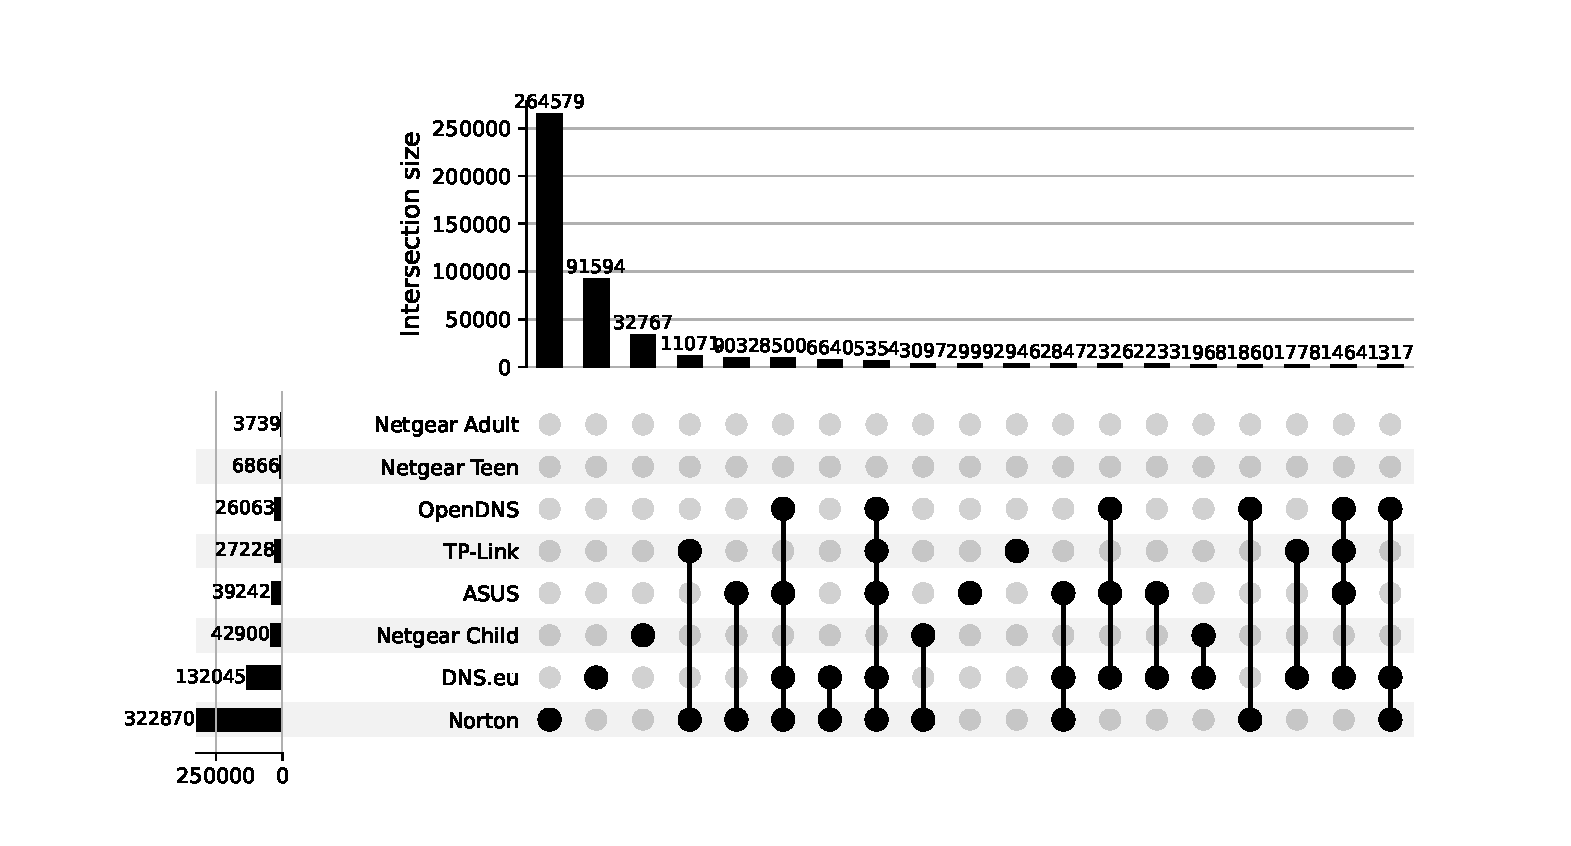
\includegraphics[width=0.95\columnwidth]{Images/Results/upset_blocked_domains_over300.pdf}
    \caption{Overlap in Blocked Domain Across Parental Control Solutions}.
    \label{fig:upset_plot}
\end{figure}

Figure~\ref{fig:upset_plot} presents an UpSet plot showing the intersection of blocked domains across all parental control systems analyzed in this study. We show only intersections containing more than 300 domains for better visibility. Netgear Adult is the only exclusive set not represented in this graph, due to its small size (21).
Each bar represents a group of domains blocked by the combination of systems indicated by the dots below. If a column contains a single dot, it corresponds to the set of domains blocked exclusively by the associated parental control system.
The largest set (264,579) consists of domains blocked only by Norton, highlighting it as the most restrictive tool among those measured.
DNS.eu follows with 91,594 blocked domains exclusively by its filtering system.
The distinctiveness of these exclusive sets highlights how these two tools enforce restrictions more independently and strictly than the others.
Most of the largest intersections involve Norton, which is expected, as it has the largest number of blocked domains.
Notably, Netgear Child, Teen and Adult, rarely overlap, further reflecting the inconsistent blocking behaviors observed in the previous analysis.
Although too small to be clearly visible in the plot, only 205 domains are blocked by all eight parental control solutions, illustrating the lack of alignment across tools and the absence of a unified approach to blocking content.

\textit{Key takeaway: The majority of solutions perform better with adult content domains than other sensitive categories. However, over-blocking in non-sensitive categories is often present. Additionally, more restrictive settings do not automatically mean safer blocking and can lead to inconsistency.}

%\todo[inline]{Antonia: Do we need the following part?}

 

\section{Discussion}\label{sec:discussion}
Our analysis reveals significant variation across parental control systems in both scope and strategy. 
Norton and DNS-based tools exhibit the broadest and most assertive filtering, blocking hundreds of thousands of domains, including many that are uniquely targeted by them.
In contrast, router-based solutions demonstrate more limited coverage and, in some cases, internal inconsistencies that undermine their tiered structure.
TP-Link’s keyword-based blocking shows success in specific categories but lacks broader effectiveness. 
The lack of consensus across tools, shown in both the UpSet plot and category-level analysis, highlights the fragmented nature of web content filtering.
These findings raise important questions about transparency, policy alignment, and the user’s ability to make informed decisions when selecting parental control solutions.

Our analysis is subject to a few limitations. 
First, our evaluation relies on a third-party domain classification system, in this case Cisco Umbrella Investigate, to assign categories to websites. 
While Cisco Umbrella Investigate provides a broad and well-maintained categorization, a number of domains (22\%) remained unclassified or were labeled as ``unknown''. This inherently creates a level of uncertainty as we are not able to judge if those domain should be blocked or not. 
However, it should be noted that the vast majority of unknown domains appeared in the final third of the ranked domain list, meaning they are less popular and less frequently accessed. Consequently, their impact on the overall results, particularly concerning popular domains, is considered to be limited.
%
Secondly, we have further grouped the website categories in those that should be blocked and those that should not.
This division was guided by prior literature and common sense, but it clearly contains a degree of subjectivity. 
Different stakeholders, such as parents, educators, policy makers, and parental control manufacturers may disagree on what content should be considered acceptable for different age groups.
%
% Thirdly, the scope of our study is limited to a representative but incomplete sample of parental control solutions. 

% We tested three consumer routers (one with three levels of filtering), two DNS-based services, and one software-based system. 
% This selection gave us insight on a variety of enforcement strategies, but it does not cover the full range of available tools. 
% In particular, ISP-level controls, mobile apps, and newer AI-based filtering systems were not analyzed in this instance.
% \todo[inline]{something else?}

\todo[inline]{Ale: we actually did more than one measurement, no? This was the case at least for the Cisco classification. Saying "one shot" is really dangerous.}
Thirdly, we performed a one-shot measurement to assess the blocking behavior of the selected parental control solutions. This approach gives us an overview of the overall behavior of the parental control systems we selected, but it does not allows us to draw conclusions about possible changes over time of the blocking behavior. A longitudinal study capturing updates in filtering behavior and changes in classification could provide insight into whether the effectiveness of these tools changes.

Finally, we have worked with the version of the Tranco list that does not include subdomains. This means that parental control solutions could potentially react differently to a root domain and a subdomain. We leave this analysis as future study.

% Finally, there are a number of additional performance metrics that we have deemed out of scope for this study, but that could potentially play a role, at the network level, in parental control systems, such as for example latency or the interplay between inappropriate content and security. 

% To address the limitations
% In regard to possible future work, there several feasible directions.
% As indicated in Sec.~\ref{sec:methodology}, our study focused on a set of market leading parental control solutions. However, we realize this ecosystem is in continuous evolution. In particular, our study could be expanded to cover a broader range of parental control systems, including ISP-level filtering solutions, mobile devices and newer AI-based tools.



% This expansion would provide a more complete overview of the landscape of parental control technologies.
% Second, our evaluation relied on a predefined set of domain categories that we subjectively determined to be appropriate or inappropriate for children. 
% Future work could involve user studies to gather input from parents, educators, or child psychologists, in order to better provide a stronger category selection. (maybe reowrd this last sentence)
% Third, although we focused on content filtering effectiveness, we did not evaluate potential side effects of these solutions, such latency and security issues. 
% A more holistic analysis could consider the impact of these aspects.
% Fourth, while our dataset focused on a large and ranked list of domains, future work could examine parental control behavior over time and using different datasets.
% A longitudinal study capturing updates in filtering behavior and changes in classification could provide insight into whether the effectiveness of these tools changes.
% Finally, improving classification coverage and accuracy in web classification remains an open challenge. 
% Using multiple classification systems or developing a custom classifier trained for child safety could reduce the number of unknowns and improve the analysis of blocking behavior.


\section{Conclusions}\label{sec:conclusions}
In this work, we conducted a measurement and analysis of parental control systems across three types of deployments: routers, DNS providers, and software. Using a classified list of domains, we assessed how each system handled inappropriate and sensitive content, revealing differences in both coverage and implementation strategies.

% While DNS-based solutions tended to offer consistent category-based filtering, router-based parental controls varied significantly, some applying keyword-based blocking rather than true content categorization. 
% The software solution we analyzed relies on an opaque blocking mechanisms, including browser extensions and potential traffic interception, but its exact mode of operation remains unclear.

Our findings show that the effectiveness of parental controls remains uneven across tools and vendors, with no single solution offering comprehensive protection, although DNS-based filtering seems to have a consistently higher efficiency. Often, high effectiveness in blocking inappropriate and sensitive content is accompanied by overblocking for all other categories, mostly among popular domains. And while one could argue that, for the sake of the children, blocking more is better, the effect this has on the general user experience and therefore the adoption of parental controls, remains unclear. In addition, we realized that an higher filtering granularity does not necessarily mean a better blocking effectiveness.
In the case of Netgear’s router-based controls, some domains blocked at lower levels of control are allowed at levels that should have been more restrictive. By comparison, a simple keyword-based solution like the one implemented by TP-Link easily outperform more complex approaches for categories like Adult Content and Gambling. These inconsistencies, combined with the lack of transparency in how filtering decisions are made, highlight the limitations of current parental control solutions, which work as a black-box without sufficient insight on their blocking strategies.

% Our measurement approach proved effective in uncovering key behavioral patterns across systems, but it remains limited in scope, as it relies on a relatively small set of representative solutions and a single domain list.
% Future research and development is essential to improve these tools' reliability and increase users trust.


In regard to possible future work, there several feasible directions. As indicated in Sec.~\ref{sec:methodology}, our study focused on a set of market leading parental control solutions. However, we realize this ecosystem is in continuous evolution. In particular, our study could be expanded to cover a broader range of parental control systems, including ISP-level filtering solutions, mobile devices and newer AI-based tools.
Finally, improving classification coverage and accuracy in web classification remains an open challenge. 
Using multiple classification systems or developing a custom classifier trained for child safety could reduce the number of unknown websites and improve the analysis of blocking behavior. 

%TODO: DO NOT FORGET ACKS
%\textbf{Acknowledgements --} CVD, Cisco 

\bibliographystyle{IEEEtran} 
\bibliography{references}  % references go in references.bib

\appendix

\subsection{Ethical Considerations}
Our measurement approach involves active measurements, both at the DNS level
(routers and DNS services) and the HTTPS level (software). We took care to
avoid undue load on the on the infrastructure of the services we were testing.
For the routers, we performed fewer than 120 DNS $requests/s$, which is
well below the number of requests a resolver is able to handle in operational
settings.
For the DNS service, taking into account that they involve open resolvers
dedicated not only to parental control functionality, we set an even more cautious
pace, limiting ourselves to 300K $requests/day$ (3.5 $requests/sec$).
Finally, the software solutions appeared not to directly rely on a back-end
infrastructure, so we did not apply any explicit pacing as the measurement is
naturally quite slow. To further limit any possible impact, we focused on a
one-shot measurement.
For website categorization we rely on data provided by Cisco. A number of
Top sites contain potentially disturbing content. During the
measurements we took care that we never visually load any of those pages. 

\end{document}
